	O bolsista apresentou em dois eventos no período em que se refere o presente relatório. O Colóquio Brasileiro de Matemática (CBM) e a Semana Integrada da Física de São Carlos (SIFSC). Apenas para o primeiro, realizado no Rio de Janeiro, foi necessário o uso da reserva técnica. Por isso, segue o pôster apresentado na página que se segue. O trabalho é complementar aos estudos assintóticos e de probabilidade realizados nos meses cobertos por este relatório.

\hspace{1cm}

\begin{tabular}{|c|c|c|c|c|c|}
	\hline
	Evento &  Sede & Data & Modalidade & Apresentação & Reserva Técnica \\
	\hline
	CBM & IMPA & 24-28/07/23 & Presencial & Pôster - Oral & Sim \\
	\hline
	SIFSC & IFSC-USP & 21-25/08/23 & Presencial & Pôster - Oral & Não \\
	\hline
\end{tabular}

\hspace{1cm}

O trabalho apresentado no CBM foi apresentado oralmente por meio de pôsteres no evento científico Colóquio Brasileiro de Matemática ocorrido de 24-28 de Julho no IMPA, Rio de Janeiro. Foram utilizadas duas diárias da reserva para a participação do colóquio.


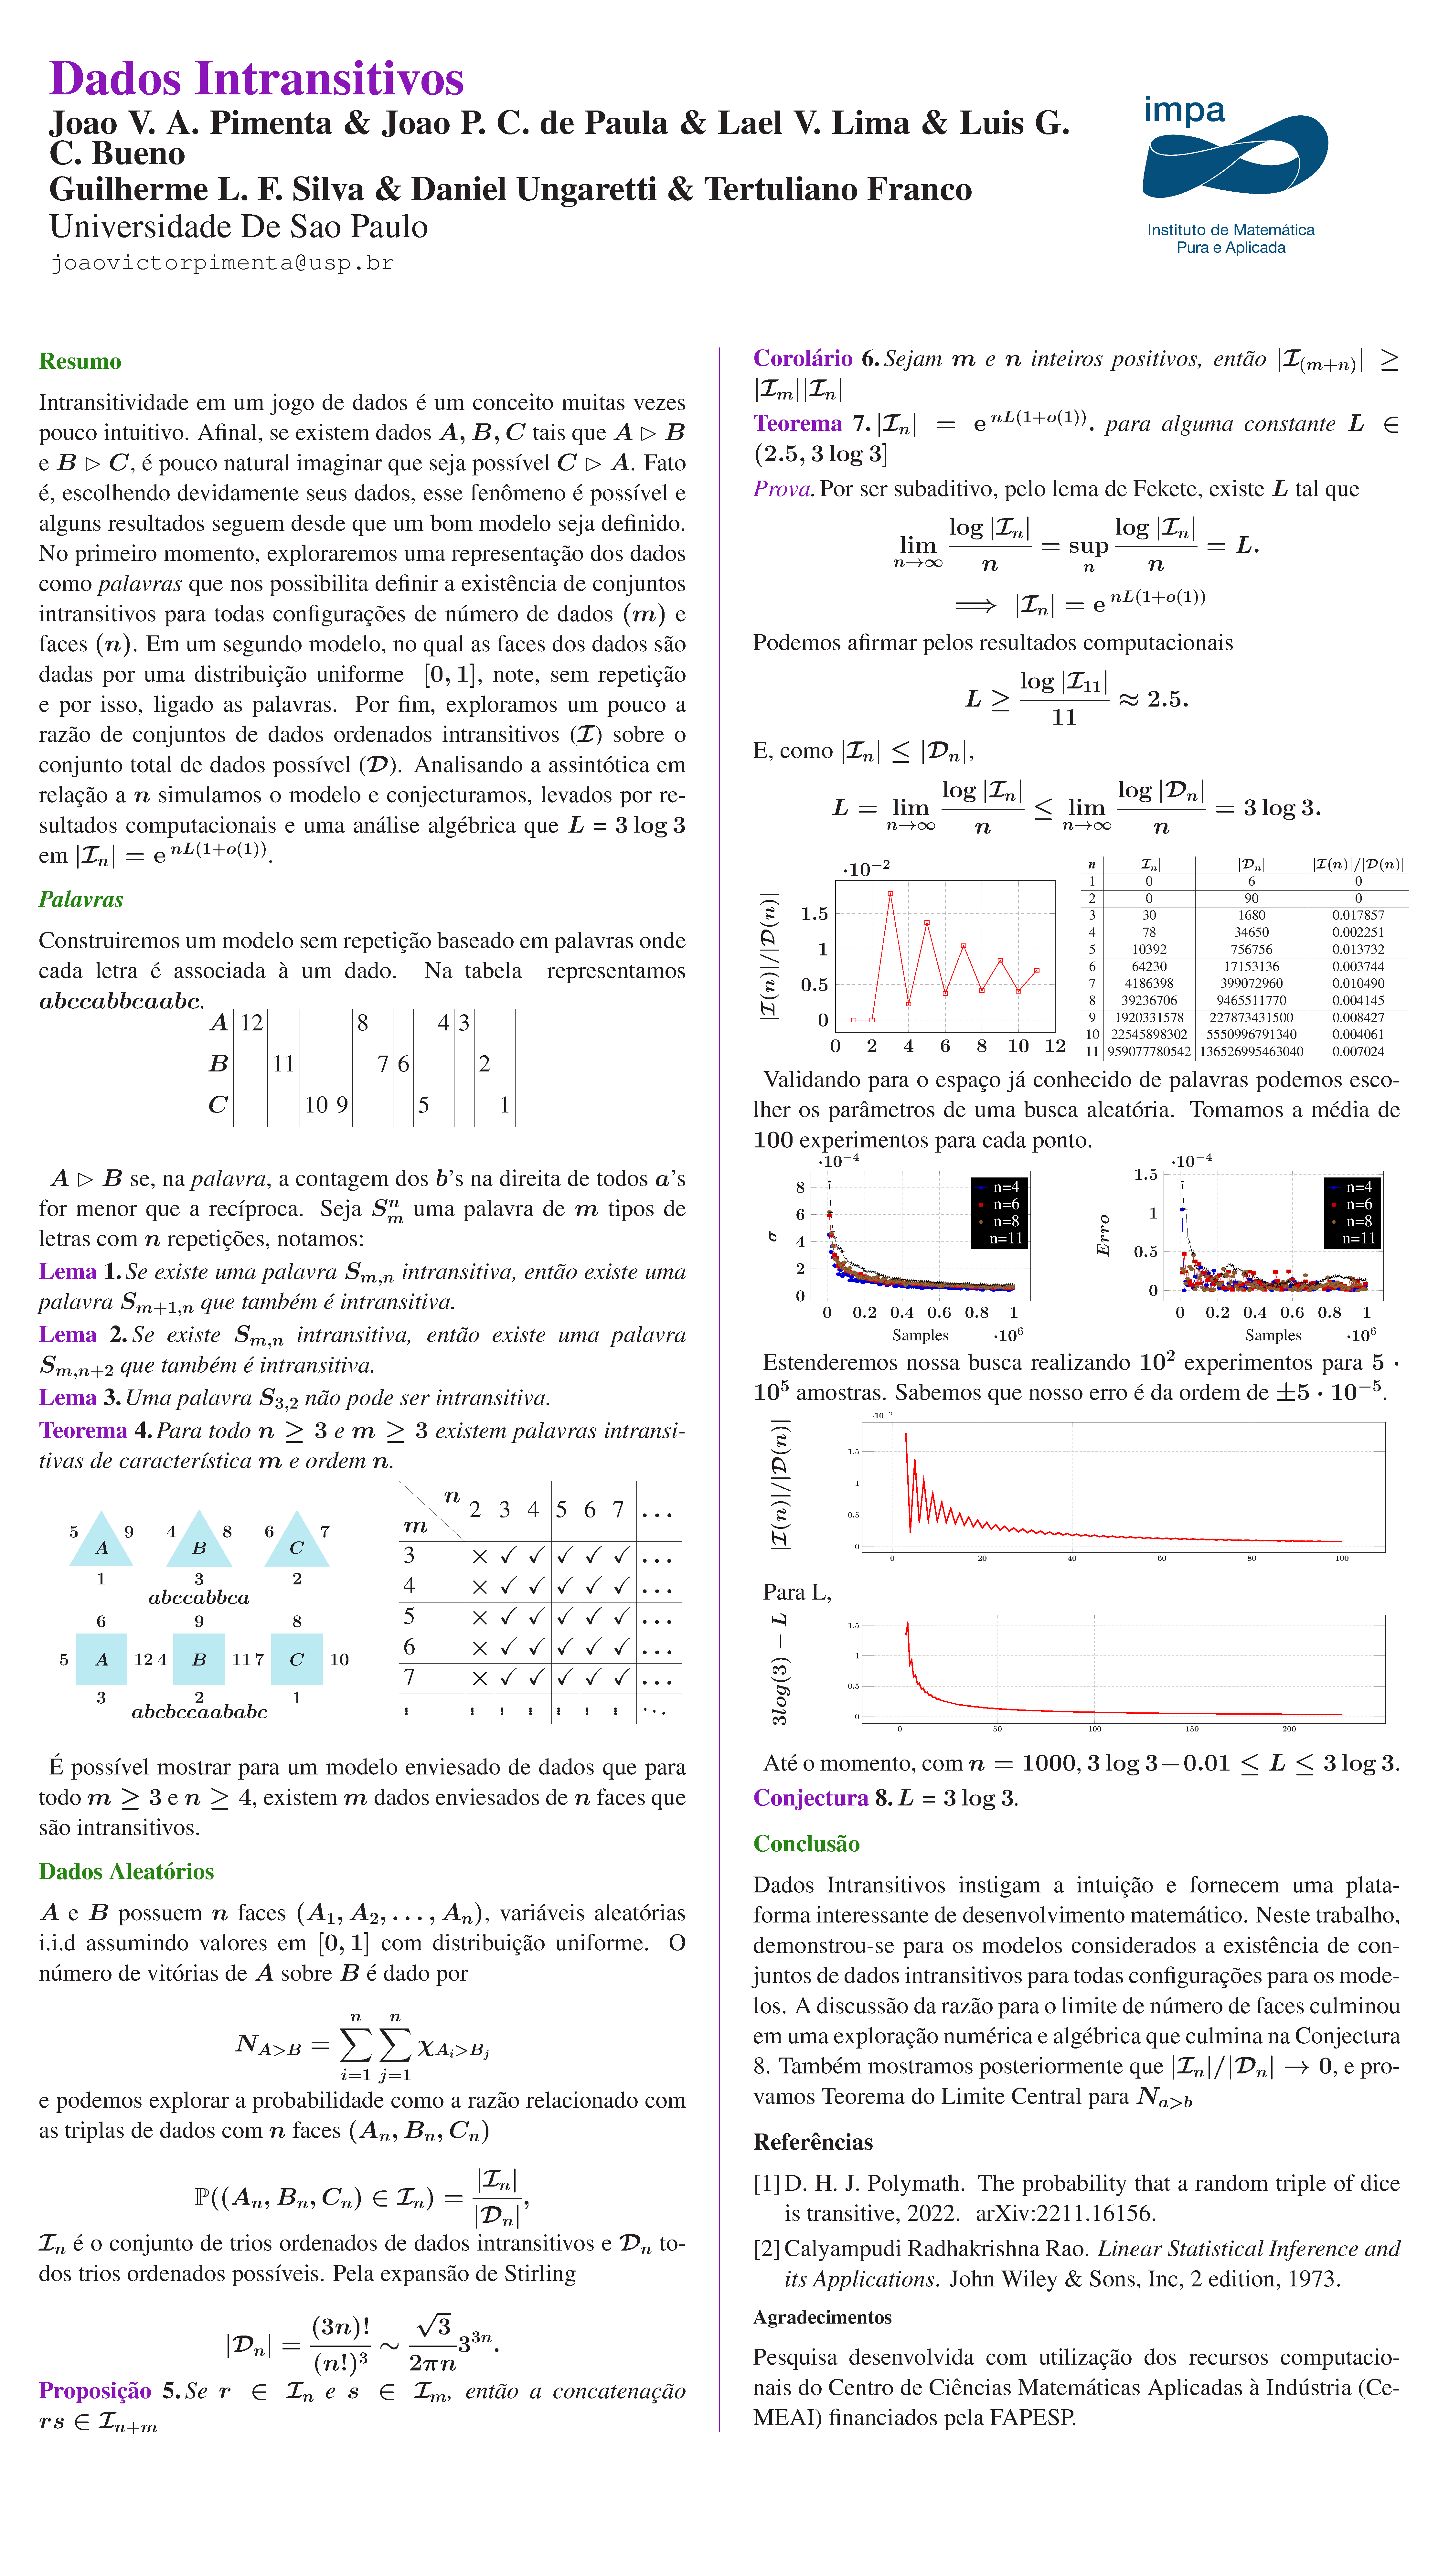
\includepdf[pages={1}]{Assets/posterwhite.pdf}